


-------------------------------------------- 5.1 --------------------------------------------
\begin{table}[h!]
\begin{tabular}{c | c}
\begin{minipage}[m]{0.4\textwidth}
\begin{tikzpicture}
        \node [anchor=south west] at (0, 0) (cartoon) {\includegraphics[width=.15\textwidth,height=.15\textwidth]{example-image-a}};
        \node [anchor=north west,rectangle callout,draw=black,
        callout absolute pointer=(cartoon.east), 
        rounded corners=3pt,text width=0.7\textwidth, inner sep=2ex] at (.19\textwidth,.125\textwidth) {This is an example.};
    \end{tikzpicture}
\end{minipage}
&
\begin{minipage}[m]{0.55\textwidth}
\begin{lstlisting}[basicstyle=\footnotesize]
\usepackage{tikz}
\usepackage[framemethod=TikZ]{mdframed}
\usepackage{xcolor}
\usetikzlibrary{calc}
\makeatletter
\newlength{\mylength}
\xdef\CircleFactor{1.1}
\setlength\mylength{\dimexpr\f@size pt}
\newsavebox{\mybox}
\newcommand*\circled[2][draw=blue]{\savebox\mybox{\vbox{\vphantom{WL1/}#1}}\setlength\mylength{\dimexpr\CircleFactor\dimexpr\ht\mybox+\dp\mybox\relax\relax}\tikzset{mystyle/.style={circle,#1,minimum height={\mylength}}}
\tikz[baseline=(char.base)]
\node[mystyle] (char) {#2};}
\makeatother
\definecolor{amber}{rgb}{1.0, 0.75, 0.0}
\definecolor{babyblue}{rgb}{0.54, 0.81, 0.94}	
\end{lstlisting}
\end{minipage}
\end{tabular}
\end{table}

%-------------------5.2
-------------------------------------------- 5.2 --------------------------------------------
\begin{table}[h!]
\begin{tabular}{c | c}
\begin{minipage}[m]{0.4\textwidth}
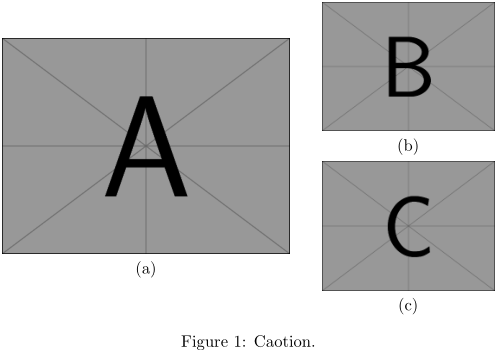
\includegraphics[width=1\linewidth]{5.2.png}
\end{minipage}
&
\begin{minipage}[m]{0.55\textwidth}
\begin{lstlisting}[basicstyle=\footnotesize]
\documentclass{article}
\usepackage{graphicx}
\usepackage{subfig}
\begin{document}
\begin{figure}[htp]
\centering
\begin{tabular}{@{}c@{}}
\subfloat{\includegraphics[width=0.5\linewidth]{example-image-a.png}}\\ (a)
\end{tabular}\qquad % some space
\begin{tabular}{@{}c@{}}
\subfloat{\includegraphics[width=0.3\linewidth]{example-image-b.png}}\\ (b)
\\[0.1cm]
\subfloat{\includegraphics[width=0.3\linewidth]{example-image-c.png}}\\ (c)
\end{tabular}
\caption{Caption.}
\end{figure}
\end{document}
\end{lstlisting}
\end{minipage}
\end{tabular}
\end{table}

\newpage
-------------------------------------------- 5.3 --------------------------------------------
\begin{table}[ht!]
\begin{tabular}{c | c}
\begin{minipage}[m]{0.4\textwidth}
 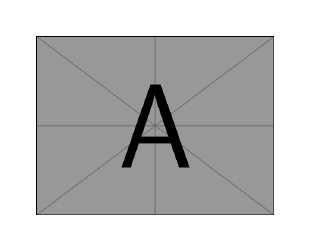
\begin{tikzpicture}
\node[ above left,
      xshift=5cm, %shifting around
      yshift=-3cm]  
{\includegraphics[width=3cm]{example-image-a.png}};
  % define destination coordinates
  \path (5,-3) coordinate (anode);
\end{tikzpicture}

\end{minipage}
&
\begin{minipage}[m]{0.55\textwidth}
\begin{lstlisting}[basicstyle=\footnotesize]
\usepackage{graphicx}
\usepackage{tikz}
\begin{document}
\begin{tikzpicture}[overlay, remember picture]
\node[anchor=north west,xshift=4cm,yshift=-11cm]
at (current page.north west) 
{\includegraphics[width=5.5cm]{example-image-a.png}};
\end{tikzpicture}
\end{document}
\end{lstlisting}
\tikz[na] \coordinate (s-anode); \xmybox[red!70!white]{place image anywhere You want}
\end{minipage}
\end{tabular}
\end{table}
\begin{tikzpicture}[overlay]
\path[->,red,thick] (s-anode) edge [bend left] (anode);
\end{tikzpicture}
-------------------------------------------- 5.4 --------------------------------------------
